

\begin{frame}[fragile]
        \frametitle{Spent Fuel Inventory}
    \begin{table}
      \centering
      \begin{tabular}{l|lll}
        \multicolumn{4}{c}{\textbf{Radioactive Waste Volumes}}\\
        \hline
Type & In storage ($m^3$) & In disposal ($m^3$)  &  \% in disposal\\
        \hline
VLLW &   2,356,000 &   7,906,000  &  77\%\\
LLW  &  3,479,000  &  20,451,000 &   85\%\\
ILW  &  460,000  &  107,000  &  19\%\\
HLW  &  22,000 &   0   & 0\%\\
        \hline
      \end{tabular}
      \caption[SNF volumes]{Solid radioactive waste volumes worldwide, IAEA
      estimate 2016. \cite{iaea_country_2015}}
      \label{tab:vol}
    \end{table}
    \end{frame}

\begin{frame}[fragile]
        \frametitle{VLLW, LLW, ILW}
        \begin{block}{Liquid}
                Must be solidified or, must be packed in absorbant package 2x liquid volume.
                (i.e. decontamination solutions, liquid scintillators, 
                ion-exchange fluids, etc.)
        \end{block}
        \begin{block}{Wet Solid}
                Greater than 1\% liquid, but primarily solid (i.e. filters).
        \end{block}
        \begin{block}{Dry Solid}
                        Less than 1\% liquid (i.e. trash, swipes, clothes, 
                        tools, etc.)
        \end{block}
\end{frame}

\begin{frame}[fragile]
        \frametitle{Spent Fuel Inventory}
                \begin{figure}[htb!]
  \begin{center}
    \includegraphics[height=0.7\textheight]{./images/fuel_assembly.eps}
  \end{center}
  \caption{Spent nuclear fuel from conventional power reactors is in the form of
    uranium oxide fuel rods \cite{nrc_nuclear-fuel.jpg_nodate}.}
  \label{fig:snf}
\end{figure}

\end{frame}

\begin{frame}[fragile]
        \frametitle{Spent Fuel}
        \begin{figure}
        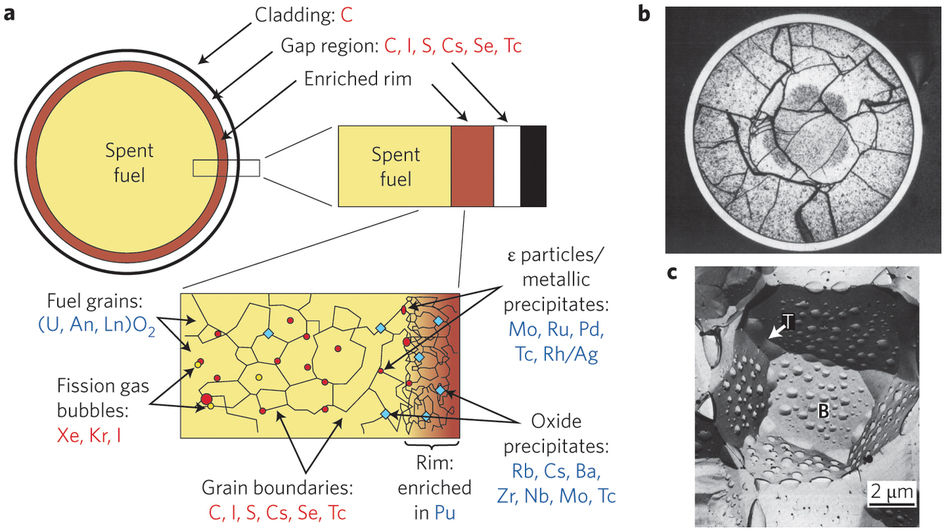
\includegraphics[width=\textwidth]{./images/ewing-microstructure}
                \caption{Microstructure of spent fuel and the distribution of
                fission products and actinides after irradiation in a reactor.
                From \cite{ewing_long-term_2015}.}
        \end{figure}
\end{frame}

\begin{frame}[fragile]
        \frametitle{Spent Fuel Inventory}
\begin{block}{High Level Waste}
        \begin{itemize}
                \item 300,000 metric tons worldwide
                        \cite{ewing_long-term_2015}
                \item 90\% in storage pools
                \item remainder in dry casks
        \end{itemize}
        \end{block}
\end{frame}

